\documentclass{article} % For LaTeX2e
\usepackage{nips15submit_e,times}
\usepackage{hyperref}
\usepackage{url}
\usepackage{graphicx}
\usepackage{amsfonts}
\usepackage{amssymb}
\usepackage{float}
\usepackage{listings}
\usepackage{xcolor}
\usepackage{amsmath}
%\documentstyle[nips14submit_09,times,art10]{article} % For LaTeX 2.09


\title{Problem Set 5 for Machine Learning 15 Fall}


\author{
Jingyuan Liu\\
AndrewId: jingyual\\
\texttt{jingyual@andrew.cmu.edu} \\
}


\newcommand{\fix}{\marginpar{FIX}}
\newcommand{\new}{\marginpar{NEW}}
\newcommand{\argmin}{\arg\!\min}
\newcommand{\norm}[1]{\left\lVert #1 \right\rVert}
\newcommand{\abs}[1]{\left\lvert #1 \right\rvert}
\newcommand{\inner}[1]{\left\langle #1 \right\rangle}

\nipsfinalcopy % Uncomment for camera-ready version


\begin{document}
\maketitle



\section{Gaussian Graphical Model}


\subsection{Derive $\phi_{ij} (x_i, x_j)$ and $\phi_i (x_i)$}

\begin{equation}
P(X \mid \mu, \Sigma) = \frac{1}{\sqrt{(2\pi)^n \Sigma}}
exp (-\frac{1}{2} (x-\mu)^T \Sigma^{-1} (x-\mu))
\end{equation}

\begin{equation}
P(X \mid \mu, \Omega) \propto exp (-\frac{1}{2} X^T \Omega X + (\Omega \mu)^T X)
\end{equation}

\begin{equation}
\qquad \qquad =
\prod_{i \in V} exp (-\frac{1}{2} x_i^T \Omega_{ii} x_i + (\Omega \mu)_i^T x_i)
\prod_{(i, j) \in E} exp( -\frac{1}{2} x_i^T \Omega_{ij} x_j)
\end{equation}

\begin{equation}
\psi_{ij} (x_i, x_j) =
exp( -\frac{1}{2} x_i^T \Omega_{ij} x_j)
\end{equation}

\begin{equation}
\psi_{i} (x_i) =
exp (-\frac{1}{2} x_i^T \Omega_{ii} x_i + (\Omega \mu)_i^T x_i)
\end{equation}

\subsection{Prove $(i,j ) \notin E \iff X_i \perp X_j | X_{V\backslash\{i,j\}}$}
If $(i, j) \notin E$, there is no edge between node i
and node j, then we can get:

\begin{equation}
\Omega_{ij} = 0, \qquad \psi_{ij} (x_i, x_j) = 1
\end{equation}

\begin{equation}
P (x_i, x_j \mid V\backslash\{i,j\}, \mu, \Omega) = \psi_{ij}' (x_i, x_j)
= \psi_{ij} (x_i, x_j) \cdot \psi_i (x_i)^{\frac{1}{n(i)}}
\cdot \psi_j (x_j)^{\frac{1}{n(j)}}
\end{equation}

\begin{equation}
=
\psi_i (x_i)^{\frac{1}{n(i)}}
\cdot \psi_j (x_j)^{\frac{1}{n(j)}}
\end{equation}

\begin{equation}
\qquad \qquad \qquad \qquad =
P (x_i\mid V\backslash\{i\}, \mu, \Omega)
\cdot P (x_j\mid V\backslash\{j\}, \mu, \Omega)
\end{equation}

\begin{equation}
\qquad \qquad \qquad \qquad \quad =
P (x_i\mid V\backslash\{i,j\}, \mu, \Omega)
\cdot P (x_j\mid V\backslash\{i,j\}, \mu, \Omega)
\end{equation}

We can notice the above process could be inversed, which means if we know that
the two points are independent, we could get that there is no edge between these
two nodes. Therefore, we could prove the conclusion.



\section{Sampling}


\subsection{Inverse Sampling}
\textbf{2.1.1 Prove Inverse Sampling}

First we need to prove for y' $\in$ R, then for $0 < z'< 1$, we have:

\begin{equation}
P (h^{-1} (z) <= y') = P (inf {y: h(y) = z} < y')
\end{equation}

\begin{equation}
\qquad \qquad \qquad \quad =
P (z <= h(y')) = h (y')
\end{equation}

\begin{equation}
P(h(y) < z') = P(y < h^{-1} (z')) = z'
\end{equation}

Therefor, we could prove that inverse sampling is reasonable.

The drawback is in real application, it would require a closed form
expression of F(x), which could be untractable in some cases.

\textbf{2.1.2 Find the Cauchy distribution transfermation}

Given the density function, we could derive:

\begin{equation}
h (y) = \int_{-\infty}^y p(y') dy' = \frac{1}{2} + \frac{1}{\pi} arctan(y)
\end{equation}

\begin{equation}
y = g (z) = h^{-1} (z) = tan(\pi (z - \frac{1}{2}))
\end{equation}


\subsection{Rejection Sampling}
As described, we would see that the accpeted probability is the area of the
$\tilde{p} (z)$ curve:

\begin{figure}[!htbp]
\begin{center}
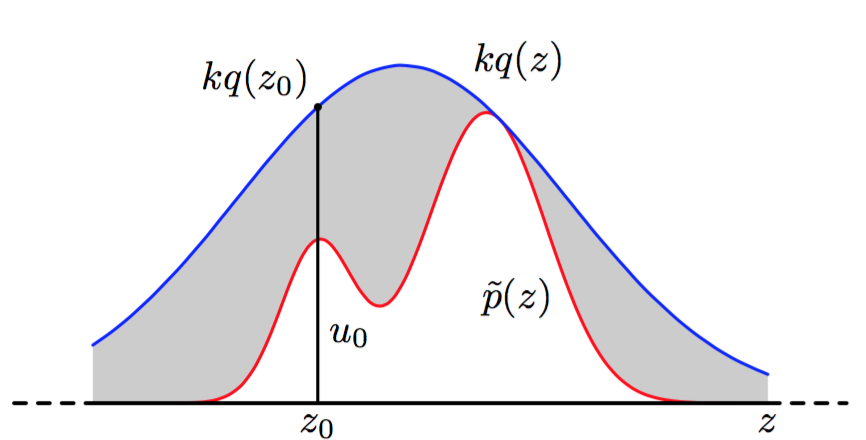
\includegraphics[width=60mm]{pic/q21.png}
\end{center}
\caption{The representation of rejection sampling}
\end{figure}

\begin{equation}
P (u_0) = P (accepted)
= \int \frac{\tilde{p} (z)}{k q (z)} q (z) dz
= \frac{1}{k} \int \tilde{p} (z) dz
\end{equation}

Based on the figure representation, we could have an intuitive prove on
the rejection sampling algorithm. Basically, we know that the k is the smallest
value to keep $kq (z) > \tilde{p} (z)$. The probability of the points that are
rejected by this method depends on the ratio of area under the unnormailized
distribution $\tilde{p} (z)$ to the area under the cureve of $kq (z)$. If the
points fall into the grey area, then it would be rejected, as it is not
generated by the $\tilde{p} (z)$.

The drawback of this rejection sampling method could be that during the sampling
iterations, the algorithms would generate too many rejected points if the real
distribution is ``small'', which would make it slow to converge.


\subsection{Markov Chain Monte Carlo}

\textbf{2.3.1 MH Algorithms}

MH is a MCMC method for obtaining a sequence of random samples. For a Markov
chain, the condition for a chain to have stationary distribution is to satisfy
the perporty of detailed balance:

\begin{equation}
p (z^{t+1}) = \sum_{z^t} T(z^{t+1}, z^t) p (z^t)
\end{equation}

\begin{equation}
p (z^{t+1}) T (z^t, z^{t+1}) = p (z^t) T (z^{t+1}, z^t)
\end{equation}

Here $T (z, z')$ is the transfer matrix or transfer condition. For the MH
algorithm, we have:

\begin{equation}
p (z^t) q (z^* | z^t) A (z^*, z^t) =
min ( p (z^t) q (z^* | z^t), p (z^*) q (z^t | z^*) )
\end{equation}

\begin{equation}
\qquad \qquad \qquad \qquad \quad =
min ( p (z^*) q (z^t | z^*), p (z^t) q (z^* | z^t) )
\end{equation}

\begin{equation}
\qquad \qquad =
p (z^*) q (z^t | z^*) A (z^t, z^*)
\end{equation}

Therefore, we could see that MH algorithm would satisfy the perporty of detailed
balance.

The drawback of MH is that this algorithm would also have
``rejection''. When we choose 1 in as the transfer value in a iteration, the new
sample is actually ``rejected''. The state of the sample point does not change
in this case.

\textbf{2.3.2 \& 2.3.3 Gibbs Sampling and Comparison with MH}

Bascially, to prove that Gibbs Sampling would achieve the p (x) stationary
distribution, we only need to prove that the Gibbs Sampling is a special case of
MH. If the essence of Gibbs Sampling is the similar to the MH, then we could
derive that it satisfy the property of detailed balance, with which we could
prove that it would converge to achieve the stationary distribution.

We could obtain Gibbs Sampling as a particular instance of MH. For a iteration,
we sample the $z_j$ while fixing the remaining $z_{\backslash j}$, so we would
have:

\begin{equation}
q_j (z^* | z) = p (z^*_j | z_{\backslash j}), \quad
z^*_{\backslash j} = z_{\backslash j}
\end{equation}

\begin{equation}
A (z^*, z) = \frac{p (z^*) q_j (z | z^*)}{p (z) q_k (z^* | z)}
\end{equation}

\begin{equation}
\qquad \qquad \qquad \qquad \qquad =
\frac{p (z^* | z^*_{\backslash j}) p (z^*_{\backslash j}) p (z_k | z^*_{\backslash j})}
{p (z | z_{\backslash j}) p (z_{\backslash j}) p (z^*_k | z_{\backslash j})}
= 1
\end{equation}

Therefore, we would know that the Gibbs Sampler is the special case of MH, with
the transfer value always 1 and accepted. Intuively, we could see that in Gibbs
Sampling, we would only change one ``dimension'' of the data state in one
iteration.

In this case, we would know that the Gibbs Sampler would not suffer from the
problem as the MH algorithm. The Gibbs Sampler would not be ``rejected'' in each
iteration, since the accepted value is always 1. However, in each iteration, the
sampling would only change one ``dimension'' of the data state.



\section{Expectation Maximization and Variational Inference}


\subsection{EM}

\textbf{3.1.1 Prove Equation}

\begin{equation}
ln p (x | \theta) = ln p (x,z | \theta) - ln p (z | x, \theta)
\end{equation}

\begin{equation}
\qquad \qquad \qquad \qquad \qquad \qquad =
ln p (x,z | \theta) - ln q (z) - (ln p (z | x, \theta) - ln q (z))
\end{equation}

\begin{equation}
\qquad \qquad \qquad \qquad \qquad =
\int_z q (z) ln \frac{p (x,z | \theta)}{q (z)} -
\int_z q (z) ln \frac{p (z | x,\theta)}{q (z)}
\end{equation}

\begin{equation}
\qquad =
L (q, \theta) + KL (q || p)
\end{equation}

\textbf{3.1.2 E-Step Maximization}

In the E-step, we can find if $q (z) = p (z | x, \theta)$, then
$KL (q || p) = 0$. Therefore, in this E step, the $L (q, \theta)$ is maximized.

\textbf{3.1.3 M-Step Maximization}

In the M-step, if we fix $q (z)$, the $KL (q||p)$ would not change, since p and
q are fixed. We know $ln p (x | \theta) = L (q, \theta) + KL (q||p)$, so if KL would
not change, and L was maximized, thus, the $ln p (x | \theta)$ was maximized.


\subsection{VI}

\textbf{3.2.1 Prove the Equation}
\begin{equation}
L (q) = \int \prod_k q_k (z_k) \{ ln p (x, z) - \sum_k q_k (z_k) \} d z_k
\end{equation}

\begin{equation}
\qquad \qquad \qquad \qquad \qquad \qquad =
\int q_k \{ \int ln p (x,z) \prod_{k \neq j} q_j dz_j\} d z_k -
\int q_k ln q_k d z_k + const
\end{equation}

\begin{equation}
\qquad \qquad \qquad \qquad \qquad \qquad =
\int q_k (z_k) E_{k \neq j} [ ln p (x,z) ] dz_k -
\int q_k (z_k ) ln q_k (z_k) d z_k + const
\end{equation}

\textbf{3.2.2 Prove the Optimal}

First we could see the first iterm $E_{k \neq j} [ ln p (x,z) ] dz_k + const$ as
a new distribution $m (x,z)$, then we wcould treat the L (q) as the the KL
divergence between $m (x,z)$ and $\{q_j\}_{j \neq k}$. Then if we fix
$\{q_j\}_{j \neq k}$, maximizing L is the same to minimize the KL divergence.

To minimize the KL divergence, we would know that when the two distributions are
the same, the KL divergence are the smallest, therefore, we have:

\begin{equation}
E_{k \neq j} [ ln p (x,z) ] dz_k + const =
ln q_k^* (z_k)
\end{equation}



\section{HMM}

\subsection{Comparison}

1. We should place $<$ here, the first item is smaller than the second item

To prove it, we could view the left as $P(A,B)$, the right as $P(A | B)$. The
$P(B)$ is smaller than 1. So the left item is smaller than the right item.

2. We should place $<$ here, the first item is smaller than the second item

To prove it, we could calculate the different part of the two probability. For
the first item, p = 0.3 * 0.7 * 0.1 + 0.7 * 0.3 * 0.2. For the second item,
p' = 0.7 * 0.1. So we could see the first item is smaller than the second.

3. We should place $=$ here, the first item is the same with the second item

To prove it, we could view the left as $P(A,B)$, the right as $P(A | B)$. The
$P(B)$ is the same with 1. So the left item is the same with the right item.

4. We should place $<$ here, the first item is smaller than the second item

To prove it, we could calculate the different part of the two probability. For
the first item, p = (0.2 + 0.1) * 0.1. For the second item, p' = 0.4 * 0.6.
So we could see the first item is smaller than the second.


\subsection{Prove the Equation}

\begin{equation}
p (x_1, x_2, ..., x_i, z_i) = p (x_i | x_1, x_2, ..., x_{i-1}, z_i)
\cdot p (x_1, x_2, ..., x_{i-1}, z_i)
\end{equation}

Because of the Markov property, we would know $x_i$ is only related to $z_i$.
So we would have $p (x_i | x_1, x_2 ,.., z_i) = p (x_i | z_i)$. Therefore:

\begin{equation}
p (x_1, x_2, ..., x_i, z_i) = p (x_i | z_i) \cdot
\sum_{z_{i-1}}p (x_1, x_2, ..., x_{i-1}, z_{i-1}) p (z_i | z_{i-1})
\end{equation}



\section{Bayesian Networks}
I found related research task stating about the DAG number of a bayes net, the
link is:

http://bnt.googlecode.com/svn/trunk/docs/usage.html\#structure\_learning

Based on its statement and prove, we would know the number $G (n)$ is:

\begin{equation}
G (n) = \sum_{k=1}^n (-1)^{k+1}
\left (
    \begin{array}{c}
        n \\
        k
    \end{array}
\right )
2^{k (n-k)} G (n-k)
\end{equation}


\section{Collaboration}
I discussed with Zheng Chen with Problem 4 and 5.



\end{document}
